\documentclass[10pt,conference]{IEEEtran}

\usepackage{cite}
\usepackage{amsmath,amssymb,amsfonts}
\usepackage{algorithmic}
\usepackage{graphicx}
\usepackage{textcomp}
\usepackage{xcolor}
\usepackage{xspace}
\usepackage{multirow}
\usepackage{subcaption}
\usepackage{tabularx}
\usepackage{booktabs}
\def\BibTeX{{\rm B\kern-.05em{\sc i\kern-.025em b}\kern-.08em
    T\kern-.1667em\lower.7ex\hbox{E}\kern-.125emX}}

\newcommand{\evpi}{Bug-AutoQ\xspace}

\newcolumntype{P}[1]{>{\centering\arraybackslash}p{#1}}
\newcolumntype{M}[1]{>{\centering\arraybackslash}m{#1}}

\begin{document}

\title{Automatically Selecting Follow-up Questions for Deficient Bug Reports}



\author{
\IEEEauthorblockN{}
\IEEEauthorblockA{Double Blind}

%\author{\IEEEauthorblockN{Mia Mohammad Imran}
%\IEEEauthorblockA{\textit{Virginia Commonwealth University}\\
%Richmond, Virginia, U.S.A. \\
%imranm3@vcu.edu}
%\and

%\IEEEauthorblockN{Agnieszka Ciborowska}
%\IEEEauthorblockA{\textit{Virginia Commonwealth University} \\
%Richmond, Virginia, U.S.A. \\
%ciborowskaa@vcu.edu}
%\and

%\IEEEauthorblockN{Kostadin Damevski}
%\IEEEauthorblockA{\textit{Virginia Commonwealth University} \\
%Richmond, Virginia, U.S.A. \\
%kdamevski@vcu.edu}
}

\maketitle

\begin{abstract}
% quality bug reporting is important
The availability of quality information in bug reports that are created daily by software users is key
to rapidly fixing software faults.
%
% Despite the success of efforts to make bug reporting consistent and detailed, numerous bug reports still lack
% sufficient important information.
%
Improving incomplete or deficient bug reports, which are numerous in many popular and actively developed open source software projects, can make software maintenance more effective and improve software quality.
%
In this paper, we propose a system that addresses the problem of bug report incompleteness by automatically posing follow-up questions, intended to elicit answers that add value and provide missing information to a bug report.
%
Our system is based on selecting follow-up questions from a large corpus of already posted follow-up questions on GitHub.
%
% To find adequate follow-up questions we use a combination of information retrieval and deep neural networks.
% %
% Using information retrieval we retrieve a candidate set of follow-up questions, while neural networks is responsible for estimating the improvement in the quality of a bug report when an answer for a follow-up question is provided.
%
To estimate the best follow-up question for a specific deficient bug report we combine two metrics based on: 1) the compatibility of a follow-up question to a specific bug report; and 2) the utility the expected answer to the follow-up question would provide to the deficient bug report.
%
Evaluation of our system, based on a manually annotated held-out data set, indicates improved
performance over a set of simple and ablation baselines.
%
A survey of software developers confirms the held-out set evaluation result that about half of the selected follow-up questions are considered valid. The survey also indicates that the valid follow-up questions are useful and can provide new information to a bug report most of the time, and are specific to a bug report some of the time.

\end{abstract}

\begin{IEEEkeywords}
follow-up questions, bug reporting, bug triage
\end{IEEEkeywords}

\section{Introduction}

In many popular software projects, bug reports arrive with frequency and in bursts that can overwhelm even well-resourced and well-organized bug triage.
%
At the same time, numerous bug reports lack sufficient actionable information for bug triagers to reproduce the bug.
%
Practitioners and researchers have observed this problem of bug report inadequacy, reporting that over 60\% of bug reports lack any steps to reproduce and over 40\% lack any description of the expected behavior~\cite{chaparro17detecting}.
%
While some software projects publish bug reporting guidelines (e.g., specific templates bug reports must follow), there are many cases where such guidelines are not followed and numerous cases where bug reports still lack crucial context or detail.
%
Bug triagers posing quick follow up questions in order to elicit additional information from bug reporters is one method to augment the bug reports with necessary information.
%
However follow-up questions are only effective if they are posed quickly, before the bug reporter loses focus on the specific bug.
%
In this paper, we examine how the posing such follow-up questions for inadequate bug reports can be performed automatically, designing and describing a system to reduce bug triage effort and improving overall bug report quality by automatically posing follow-up questions for inadequate bug reports.

\begin{figure}[ht]
\centering
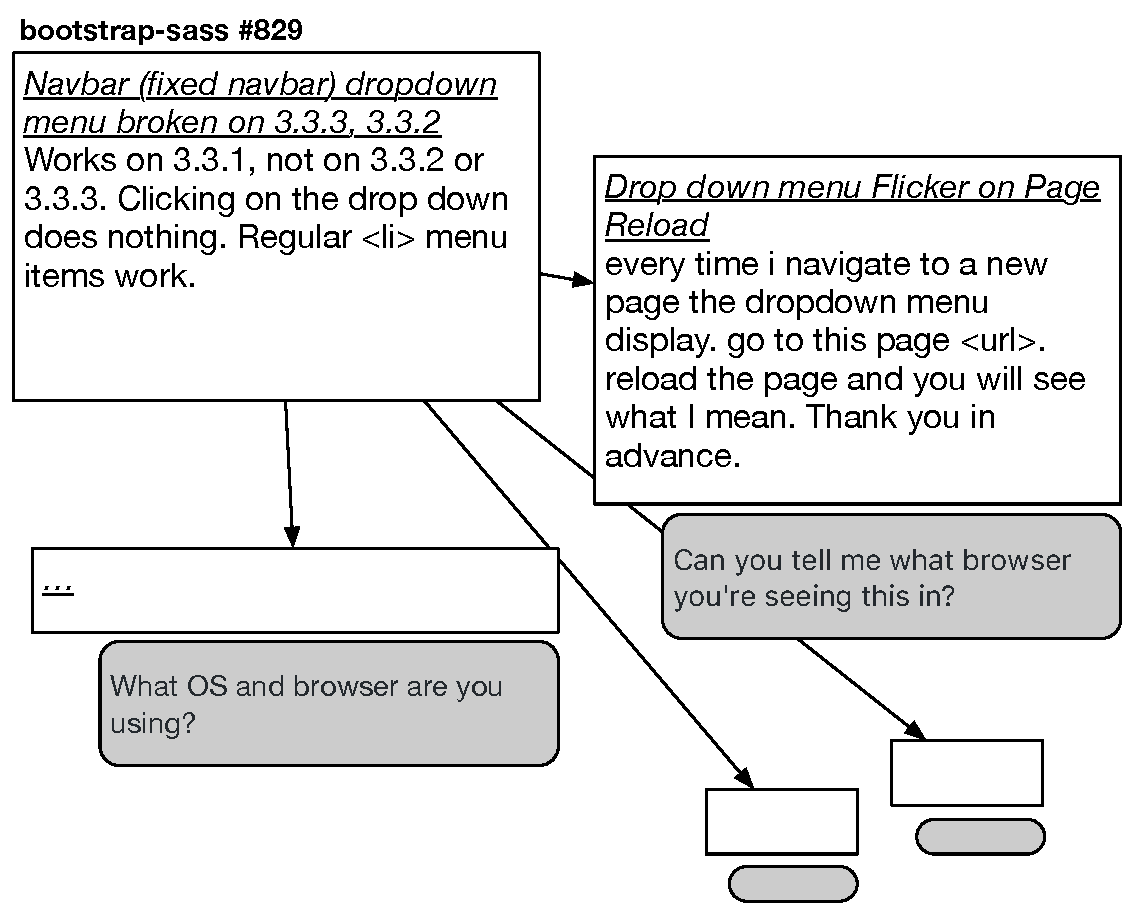
\includegraphics[width=0.99\linewidth]{figures/br_motivation.pdf}
\caption{The text for bug report (\#829) of the bootstrap-sass project is similar to other bug reports with posed follow-up questions. These follow-up questions could be recommended for this bug report.}
\label{fig:repo_activity}
\end{figure}


%
We base our automatic follow-up question posing system on the idea that: 1) relevant follow-up question are common and have already been posed in other prior bug reports, in the current project or in others; 2) similar bug reports necessitate similar follow-up questions; and 3) the utility of the answer provided to a prior similar follow up question is indicative of its value to the current bug report.
%
Therefore the task our system performs is to retrieve the most relevant and useful follow-up question for a specific inadequate bug report, given a large corpus of previous bug reports, follow-up questions, and their answers.
%
For instance, consider the example shown in Figure 1, where the bug report ....

To curate a corpus of prior bug reports, follow-up questions, and answers we leverage GitHub, where we focus on popular repositories that have a high level of activity and therefore a likely to have utilized the follow-up questions mechanism. We look for follow-up questions that have been posed in comments and gather answers that occur as comments or as edits to the original bug report text. To estimate the utility of an answer we use the patterns to identify Observable Behavior (OB), Expected Behavior (EB) and Steps to Reproduce (S2R), published by Chaparro et al. We evaluate our prototype in two ways, based on the ability to predict an annotated held-out set of follow-up questions, and based on a developer survey that aims to gage the perceived value of specific follow up questions. The results indicate that the techniques is viable, with X MRR on the held-out set and Y\% of respondents indicating that the follow-up question is “bla bla bla”.

Relative to the prior efforts by the software engineering research community towards improving the quality of bug reports, this paper is the first to use follow-up questions and to propose a specific mechanism for this purpose. Automatically posing follow-up has been used in other domains for improving the quality of Web forum posts~\cite{rao-daume-iii-2018-learning}, product reviews in online retail, and improving query quality in Web search.

% More specifically, the contributions of this paper are:
%
% \begin{itemize}
% \item x
% \item y
% \item z
% \end{itemize}


\section{Bug Reporting in Open Source Projects}


%The problem is real, i.e., there are repos that have more BRs than they can manage. How many BRs arrive at the most popular repos (is the traffic bursty)? how many lack OB/EB/S2R from these?
The overall trend in software development in recent years is towards increased
speed of development and delivery. There are nowadays numerous projects on popular
public software collaboration platforms like GitHub that have large development
teams and user communities. Many of these projects experience significant
bug reporting traffic~\cite{Zhang2014ASO}. Figure~\ref{fig:repo_activity} shows the issue creation
frequency for a selection of ten GitHub repositories that are currently active
with a high numbers of commits and developers. Three of these repositories have
a median of over 40 issues created daily, where most of them are bug reports reported by
GitHub identities that have not contributed to the project (i.e., users). In addition,
the same three projects exhibit high variance in daily issue creation, likely indicative
of bursty and hard to predict bug reporting activity. This is a
considerable burden for bug triagers and it motivates the need for the type of work
as described in this paper, which intends to make bug triage more efficient and less of
a burden for project maintainers.


\begin{figure}[t]
\centering

\includegraphics[width=0.99\linewidth]{figures/bug_report.pdf}
\caption{Bug report with follow-up question and OB in answer.}
\label{fig:bug_report}
\end{figure}

% The preconditions are present, i.e., there are a lot of follow-up questions on GitHub -- we could
% use the same set of 10 repos to show this.
Posing follow-up questions is an already practiced mitigation strategy for deficient bug
reports. To lend support for this claim and to quantify how widespread is the use of
follow-up questions, we performed a small scale study of the prevalence
of follow-up questions on GitHub, focusing on the 10 active projects used in Figure~\ref{fig:repo_activity}.
From each of the 10 repositories, we randomly sampled 50 closed bug reports (500 in total) and manually examined them
for follow-up questions. We were also interested whether the answers to those questions (if they are present) provide any
of the three key parts of a bug report: Observable Behavior (OB), Expected Behavior (EB) or Steps to Reproduce (S2R).
We found that follow-up questions were present in 23.6\% (118/500) of bug reports and about 73\% (86/118) of them were
answered with 57\% (49/86) of the answers containing Observable Behavior, Expected Behavior or Steps to Reproduce.

We highlight one of the bug reports we examined ({\bf ansible/ansible \#3933}) in Figure~\ref{fig:bug_report}. The follow-up question {\em What OS/version of
Ansible was this on?} elicited an answer that provided key OB to this bug report, leading to its quick subsequent fix.
Developer surveys have confirmed the importance of OB, EB and S2R in bug reports , noting that S2R is among the most valuable aspects of a bug report
with OB and EB closely behind~\cite{zimmermann10whatmakes,laukkanen2011survey}. The availability of existing follow-up questions on social coding platforms like GitHub provides the preconditions for the approach described in this paper, which leverages such existing follow-up questions to automatically rank and select the most appropriate one to be asked for a newly written, incomplete bug report. In the remainder of this paper, we describe the design of this system, which we entitle \evpi\ -- Bug Incompleteness Questioner\footnotemark\footnotetext{Replication package available at: https://tinyurl.com/y223uva2}.


\section{System Description}

% describe overall system
As input, our system for retrieving follow-up questions requires: 1) an incomplete bug
report of interest; 2) a corpus of already posed follow-up questions extracted
from GitHub issues, including their corresponding bug reports and answers. As output, our system
produces a ranked list of follow-up questions appropriate to the deficient bug report.
In this section, we describe our system, including how we create
a large corpus of follow-up questions to recommend, how we select candidate follow-up questions from
this corpus for a specific incomplete bug report, and how we rank these questions in descending order of
their potential utility to the bug report.

\subsection{Selecting a Corpus of Bug Reports}


\begin{figure}[b]
\centering
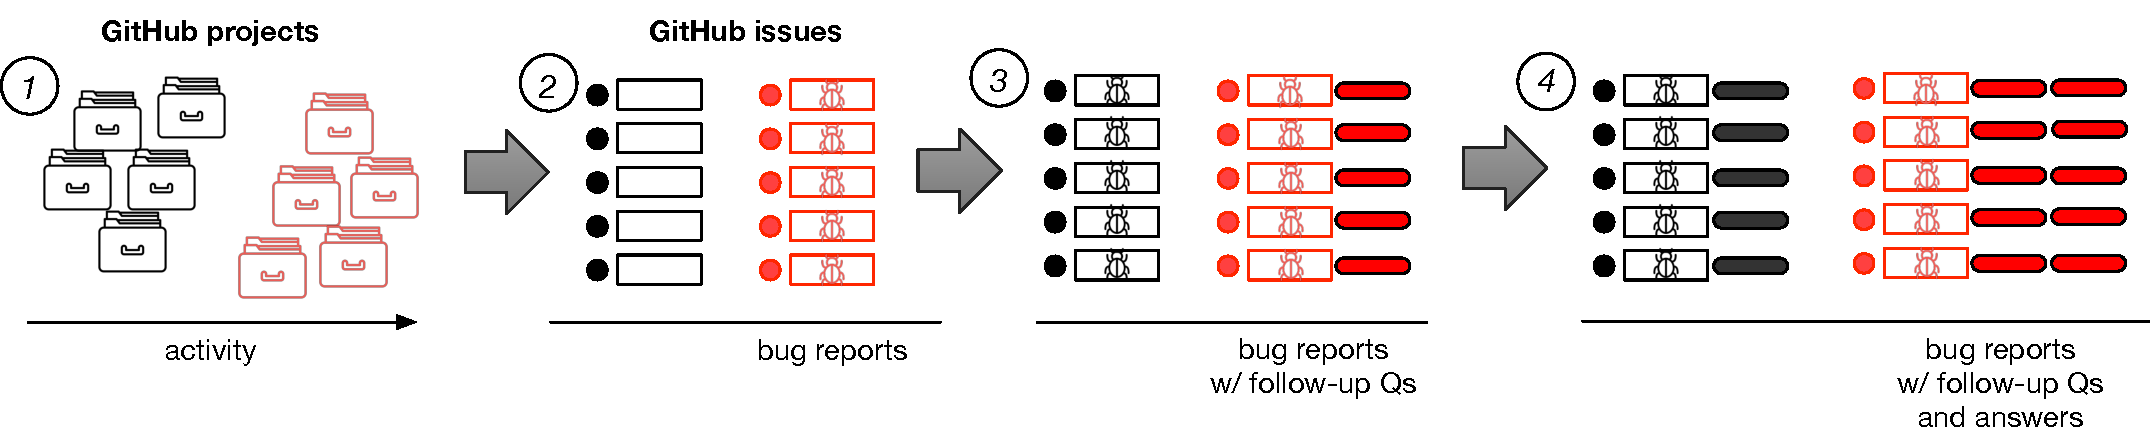
\includegraphics[width=0.99\linewidth]{figures/pipeline.pdf}
\caption{Automatically curating a input corpus for our system follows a sequence of filtering steps, starting with filtering
GitHub repositories to selecting only the issues in these repositories that are bug reports with answered follow-up questions.}
\label{fig:pipeline}
\end{figure}

% overview of the entire process
Our goal in curating a corpus of bug report-related follow-up questions and their answers
is to find a large, representative and high-quality corpus. Manually curated corpora are of
high quality but they are difficult to scale-up. Automatic curation can easily scale but it
can be affected by significant noise, leading to low data quality, unless care is taken
to filter and sample follow-up questions in a way that noise is mitigated. As corpus size
is an important factor in our system, we opt for an automated approach with numerous filters
to ensure the data is of highest possible quality. With the number of active repositories available
on GitHub providing a very large input domain, we can afford to err on the side of being overly
restrictive in our filtering.
To automatically curate our corpus, we: 1) select GitHub repositories that have high bug reporting activity,
as measured by the number of issues created by non-contributors over some fixed period of time; 2) select issues in those bug repositories that contain rapidly asked and succinct follow-up questions contained in GitHub issue comments; 3) locate
answers to the follow-up questions encoded as either comments or as edits to the
original bug report.

In more detail, we used the following sequence of steps to curate the corpus. The highlights of the corpus curation process are also illustrated in Figure~\ref{fig:pipeline}.
\begin{enumerate}
\item We scraped a set of public GitHub repositories with a high rate of
non-contributor created issues, where a non-contributor is a GitHub user that has never
committed any code in the specific repository. Repositories with these characteristics form
the target population of software projects that are more likely to use our technique. In order
to somewhat constrain  the amount of repositories, we focused on longer-running projects,
specifically, created between 2008-2014, and recently active with new issues created in the repository after Jan 1, 2019.
\item For each of these repositories, in their descending order of activity as defined in the previous step,
we selected issues in their GitHub issue tracker that are labeled as ``bug", ``crash", ``fix", ``defect" or unlabeled. Our goal for this step was
to avoid feature requests and focus on bug reports. We observed that issue labels were not used consistently enough
in projects, which is why we opted to include unlabeled issues. Since we are interested in incomplete bug reports, we select bug reports that do not contain Observable Behavior, Expected Behavior or Steps to Reproduce. While focusing on incompleteness in one of these categories is possible, for simplicity, we chose bug reports that lacked all three.
\item We further selected only issues that contain follow-up questions in one of the issue comments.  We identified follow-up questions as GitHub comments containing only questions, identified by both starting with an interrogative word and ending with a question mark. In order to ensure we selected follow-up questions and not just
any questions, we constrained our selection based on time and comment sequence. That is, the comment containing the follow-up question must have been posted within 60 days of the issue creation date and must have occurred as the comment immediately following the post. We also ignored follow-up posts by the issue author by ensuring that the comment was authored by a different user from the author of the issue.
\item The set of issues and candidate follow-up questions from the previous step were further filtered to
retain issues and follow-up questions where an answer was provided. A key heuristic we used for recognizing an answer was that it was authored
by the original issue creator and occurred as the the next sequential comment
to the follow-up question. We also searched for answers that were encoded as edits to the original issue text by the author, which occurred after the follow-up question was posted and were limited to add at least 4 additional words to the original text in order to avoid minor spelling or grammar modifications.
\end{enumerate}

 We stopped the collection process when we gathered a dataset of 25K GitHub issues, which we deemed to be sufficient for our purpose. Each data point in our dataset is a triple of
issue, follow-up question, and answer. Together, the 25K triples form the primary corpus we used to
retrieve and rank follow-up questions for a given incomplete bug report.


\subsection{Selecting Candidate Follow-Up Questions}

Selecting a set of most likely candidate follow-up questions for a specific incomplete bug report of interest from the corpus
of 25K triples (bug reports, follow-up questions and their answers) can be formulated as an information retrieval
problem. That is, as a query we can use the text of the incomplete bug report. We can represent the corpus
as an inverted index of the bug report text (e.g., using Lucene), and use tf*idf as the
ranking mechanism. In this way, we retrieve a set of 10 candidate follow-up questions for each incomplete bug report
of interest, where these 10 candidates have the most similar bug report text to the bug report of index.

More specifically, we create a Lucene index of the corpus of bug reports by following this set of steps:
\begin{itemize}
\item {\em Filtering.} Removing code or stack traces from bug reports in our index allows
for more accurate matching. GitHub issues use markdown so we remove all text surrounded
by triple-quotes as this is typically how source code and stack traces are encoded. We also
remove quoted text (i.e., lines that start with the greater than symbol) as these typically
refer to some external information, which, again, is often stack traces, code, or project documentation.
\item {\em Tokenization.} We perform standard tokenization used in software engineering applications
of information retrieval~\cite{marcus2004information,shepherd2012sando}. We tokenize on white space, remove
punctuation (except for horizontal dashes)
and split on camel case and dashes, while also keeping the original unsplit tokens.
\item {\em Indexing.} We use Lucene's standard configuration to index the title and the body in separate fields,
in order to ensure better quality matches, especially when the bug report body has a lot of text. In order to provide
more context, we extract the tags that the bug report is labeled with (e.g., {\em fix-later, critical}) and the tags the
GitHub repository is tagged with (e.g., {\em java, linux, web-server}). The former provides specifics on the issue while the
latter usually denotes technologies or the project uses or broad categories it belongs to.
\end{itemize}

To create a query out of the incomplete bug report, we tokenize its title and body
using the equivalent process to the one we performed on the bug reports in the corpus.
While obtaining a ranked list of follow-up questions from Lucene, we obtain and list of 10
triples and ignore the ranking. In the following section, we describe a customized ranking, which
takes more factors into account when choosing which follow-up question to pose to the deficient
bug report.


\subsection{Ranking the Candidate Follow-Up Questions}\label{sec:ranking}

To rank the set of candidate follow-up questions we reformulate and apply towards bug reporting
the notion of the Expected Value of Perfect Information (EVPI), initially proposed as a means to
rank follow-up quesitons by Rao et al.~\cite{rao-daume-iii-2018-learning}. To evaluate a follow-up question, EVPI suggests
using the (expected) value of its answer, i.e., for an
incomplete bug report, EVPI estimates the value of the information provided by the answer to the
follow-up question. The higher the EVPI the higher we rank a follow-up question from the candidate
set.

Given an incomplete bug report of interest, $br$, we express the EVPI of a specific follow-up question $q_{i}$ from our candidate set
as the product of: 1) the {\em compatibility} of a specific follow up question to the bug report, i.e.,
the probability of a specific question and answer pair occurring for that bug report, $P(q_{i}+a_{i}|br)$, and 2) the {\em utility} of that question, $U(q_{i})$.

$$EVPI(q_{i}|br) = P(q_{i}+a_{i}|br) * U(q_{i})$$

The utility of a question is further expressed in terms of the average quality of the answers it has received, i.e.,

$$U(q_{i}) = \frac{1}{|A|} * \sum_{a \in A}^{} \frac{|OB(a)|+|EB(a)|+|S2R(a)|}{|a|}$$

\noindent
,where $A$ is the set of answers $q_{i}$ has received in the corpus, $a$ is one of those answers, and
$OB(a)$, $EB(a)$ and $S2R(a)$ are the sentences describing Observable Behavior (OB), Expected Behavior (EB), or
Steps to Reproduce (S2R) found in the answer. We use the $|\cdot|$ operator to denote the cardinality of a set.
The idea of this metric is that questions whose set of answers have a high proportion
of OB,EB, or S2R of a bug report have higher utility than do questions whose answers do not contribute much in
terms of this information.

\subsubsection{Computing Compatibility}
To compute the probability of a follow-up question occurring for a given bug report, $P(q_{i}+a_{i}|br)$, we use a neural
network approximation, using a deep NN consisting of 3 layers. As the first layer, in order to introduce semantics, we encode
the bug report text with GloVe word embeddings that we pre-trained on the entirety of Stack Overflow (using the most recent Stack Overflow data dump as of June, 2020) with default parameters. As the second layer, in order to capture the word sequence, we train a LSTM and compute an average across the hidden layer. As the third and final layer we use a 4-layer dense neural network. The output of the entire network is vector as similar as possible to the concatenation of the average word embeddings of $q_{i}$ and $a_{i}$ (using the same GloVe vectors as above). We train the neural architecture using the actually posed follow-up questions and answers as positive labeled examples for $q_{i}$ and $a_{i}$ and the remaining 9 question-answer pairs in the candidate set as negatively labeled. We use cosine embedding loss and weight balancing to manage the resulting class imbalance as the negative examples significantly outnumber the positive ones, 9 to 1.

\subsubsection{Computing Utility}
To compute the utility of the follow-up question, $U(q_{i})$, we leverage the pattern based
identification of the constituent pieces of a bug report (OB,EB and S2R) created by Chaparro et al.~\cite{chaparro17detecting}
We implement 5 of the most common and most productive patterns for each of OB,EB and S2R, as described by
the authors. Each of the total 15 patterns we implemented rely on predefined sets of keywords and part-of-speech tagging to ensure high
precision. In order to compute the average utility of the answers for a particular question in the corpus, we rely on Lucene to provide
matching between questions and we reserve 10 of the most similar question variants for each queried follow-up question.


%
% p(a_i|q_i,p_i) is estimated via a 5-layer feed-forward NN.
%
% U(p+a) = softmax(d_OB+d_EB+dS2R), where dOB = OBa_i - OBp, and similarly dEB and dS2R
%
% OB_x is the number of OB sentences in document x, as defined by Chaparro et al.


\section{Evaluation}

We implemented a prototype of the system with the aim of evaluating its efficacy along
a few different dimensions. First, we use metrics and a held-out data set to evaluate the quality
of the recommendation, i.e., how well the system selects valid follow-up questions for incomplete bug reports.
Second, we use a survey of software developers to evaluate the follow-up questions on their usefulness, novelty and specificity.


\subsection{Quality of Follow-Up Question Ranking}

One way of evaluating the ranking system, based on a held-out dataset (of bug reports and candidate follow-up questions), is
by using the posed questions as the ground truth. However, this simple setup has a serious deficiency in that the posed question
may not always be the most optimal among the set of candidate follow-up questions. More importantly, several of
the remaining candidate questions may be valid and (more) relevant to the bug report and therefore should
not be considered as negatively labeled instances for evaluation. Therefore, in order to provide an evaluation
set that identifies all of the valid questions in the candidate set, we perform manual annotation that clearly
identifies all of the valid follow-up questions for a specific bug report.

\subsubsection{Annotation}
We annotated 400 randomly chosen bug reports that were held out from our original corpus of 25K. The annotation
was performed by two of the authors following an agreed-upon predefined procedure. For each bug report, each annotator 1)
read the bug report carefully, spending a few minutes to understand its context, e.g., by looking at the purpose of the overall GitHub
project and the types of technologies it relies on; 2) marked all of the follow-up questions for the candidate set of 10
that were valid. Both of the annotators processed the same set of 400 bug reports, marking an average of 3.45/10 of the follow up questions as valid with an inter-annotator agreement (Cohen's kappa) of 0.60.
We use the set of follow-up questions that both annotators agreed were valid, i.e., the intersection between their annotation.

\subsubsection{Baselines}
The baselines we identified are meant to convey both straightforward approaches to ranking (e.g., directly using the Lucene output) and
ablation, i.e., using one part of our ranking function but not the other (e.g., ranking based only on the question utility, $U(q_{i})$).
We did not find appropriate prior research work to compare against, since the research direction is novel and models from other domains
with a similar purpose are too different in form. Below is an enumerated list of all of the ranking baselines we used.
\begin{itemize}
\item {\em Random} -- A random permutation of the candidate follow-up question list. We present metrics averaged over 10 runs.
\item {\em Lucene} -- Lucene uses the vector space model (i.e., tf*idf) to rank follow-up questions based on the similarity between the bug reports. This baseline just transfers Lucene's ranking, which we use to generate our candidate set of 10 follow-up questions, as the system's output.
\item {\em Utility only} -- $U(q_{i})$ -- The utility function, described in detail in Section~\ref{sec:ranking}, computes the average amount of OB,EB or S2R found in the answers to the specific follow-up question.
\item {\em Compatibility only} -- $P(q_{i}+a_{i}|br)$ -- The compatibility function computes the probability a bug report can be combined with a specific follow-up question and answer pair. The implementation uses a deep NN architecture to compute this quantity.
\end{itemize}

\subsubsection{Metrics}
We use a two popular information retrieval evaluation metrics: Mean Reciprocal Rank (MRR) and Precision@n (P@n).

The goal of MRR is to evaluate how effective is our technique, or a baseline, in locating the first valid follow-up question, as, presumably, this is a proxy for the ease with which an end-user would locate a follow-up question in the ranking. It is
computed as: $$MRR = \frac{1}{|B|} \sum_{i=1}^{|B|} \frac{1}{rank_{i}}$$ ,where $B$ is the set of bug reports in the test set and $rank_{i}$ is the ranked position of the first valid follow-up question for the $i^{th}$ bug report.

The goal of Precision@n is to measure the number of valid results when considering the top $n$ positions in the ranking. Unlike MRR, it consider all, not only the topmost ranked, results. It is computed as: $$P@n = \frac{1}{|B|} \sum_{i=1}^{|B|} \frac{|v|}{n}$$ ,where, as before, $B$ is the set of bug reports in the test set and $v$ is the set of valid follow-up questions ranked in the top $n$ positions. We use values of 1, 3 and 5 for $n$.


\begin{table}[t]
\centering
\caption{Evaluation results contrasting our system (\evpi) relative to several baselines.}
\begin{tabular}{p{3cm}cccc}
\hline
%                          & \multicolumn{4}{c}{$V_{1} \cap V_{2}$} \\\hline
                          & {\bf MRR}  & {\bf P@1}  & {\bf P@3}  & {\bf P@5}  \\\hline
{\em Random}              & 0.52 & 0.32 & 0.33 & 0.34 \\
{\em Lucene}              & 0.53 & 0.35 & 0.32 & 0.32 \\
{\em Utility only}        & 0.65 & 0.47 & 0.44 & 0.41 \\
{\em Compatibility only}  & 0.61 & 0.43 & 0.38 & 0.38 \\
{\em \evpi}                & 0.67 & 0.49 & 0.49 & 0.45 \\ \hline
\end{tabular}
\label{tab:results}
\end{table}


\subsubsection{Results} We summarize the results of our technique (\evpi) versus the identified
baselines in Table~\ref{tab:results}. Our results indicate that \evpi outperforms all of the baselines,
with the ablation-type baselines performing better than the simple baselines. The Lucene ranking
does surprisingly poor, basically in line with the Random baseline. The Utility only baseline is
the ones that comes closest to the performance of the full system. Perhaps the most intuitive result
is $P@1$, where \evpi scores 0.49, indicating that just about half of all of the top selected follow-up
questions by our system were valid.


\subsection{Developer Survey}
While a recommended follow-up question may be valid, it may not possess other properties that would
encourage its use in practice, i.e., in a system that automatically poses follow-up questions for incomplete bug reports. For
instance, a follow-up question may be overly generic, lacking detail or context specific to the bug report (e.g., {\em Can you provide
additional information?}). To investigate how \evpi performs across several such dimensions of interest we conducted a survey with
software developers.

%\subsubsection{Participants}
Through personal contacts, we e-mailed 10 software developers about the study, providing the basic context of our project
and a link to a Web form containing the survey. None of the developers were
aware about the details of our technique. The developers were half (5) from academia (graduate students at
institutions in the U.S. and Europe) and half professional developers from industry. All had programming
experience of 4 or more years with popular languages like Java and Python and all indicated one of their primary
responsibilities was developing software.

%Procedure
We randomly assigned the developers into two groups of 5 and each group was assigned 12 instances of bug report and follow-up question pairs, where all of the follow-up questions were the top-1 selected by \evpi. Each group was presented with bug reports from our corpus that belong to GitHub projects where Java or Python were the primary technologies used. For each one of the assigned bug reports, a developer
was presented with a screenshot from GitHub containing the title and text of the bug report, the follow-up question, and a link to the project the bug report came from for context. Prior to beginning the survey, we gave instructions to the developers to read both the bug report and the follow-up question before answering the provided set of survey questions. A preliminary survey question, which was posed on an initial screen, asked {\em Is the follow-up question valid?}. A negative response indicated that the follow-up question was invalid and unusable, so, therefore we asked no additional survey questions for that specific bug report - follow-up question pair. The remaining survey questions only appeared for instances deemed valid by a developer.

%Measures
For a valid follow-up question, we posed a yes/no survey question interrogating {\em Does the follow-up question ask for new information currently not included in the description?}, followed by two Likert score survey questions (5 point; Strongly Disagree, Disagree, Neutral, Agree, Strongly Agree) interrogating {\em The follow-up question is specific to the bug report} and {\em The follow-up question is useful to the bug report}. In the following, we refer to the first (yes/no) survey question as measuring New Information, the second measuring Specificity, and the third measuring Usefulness.

\begin{figure*}[t]
\centering
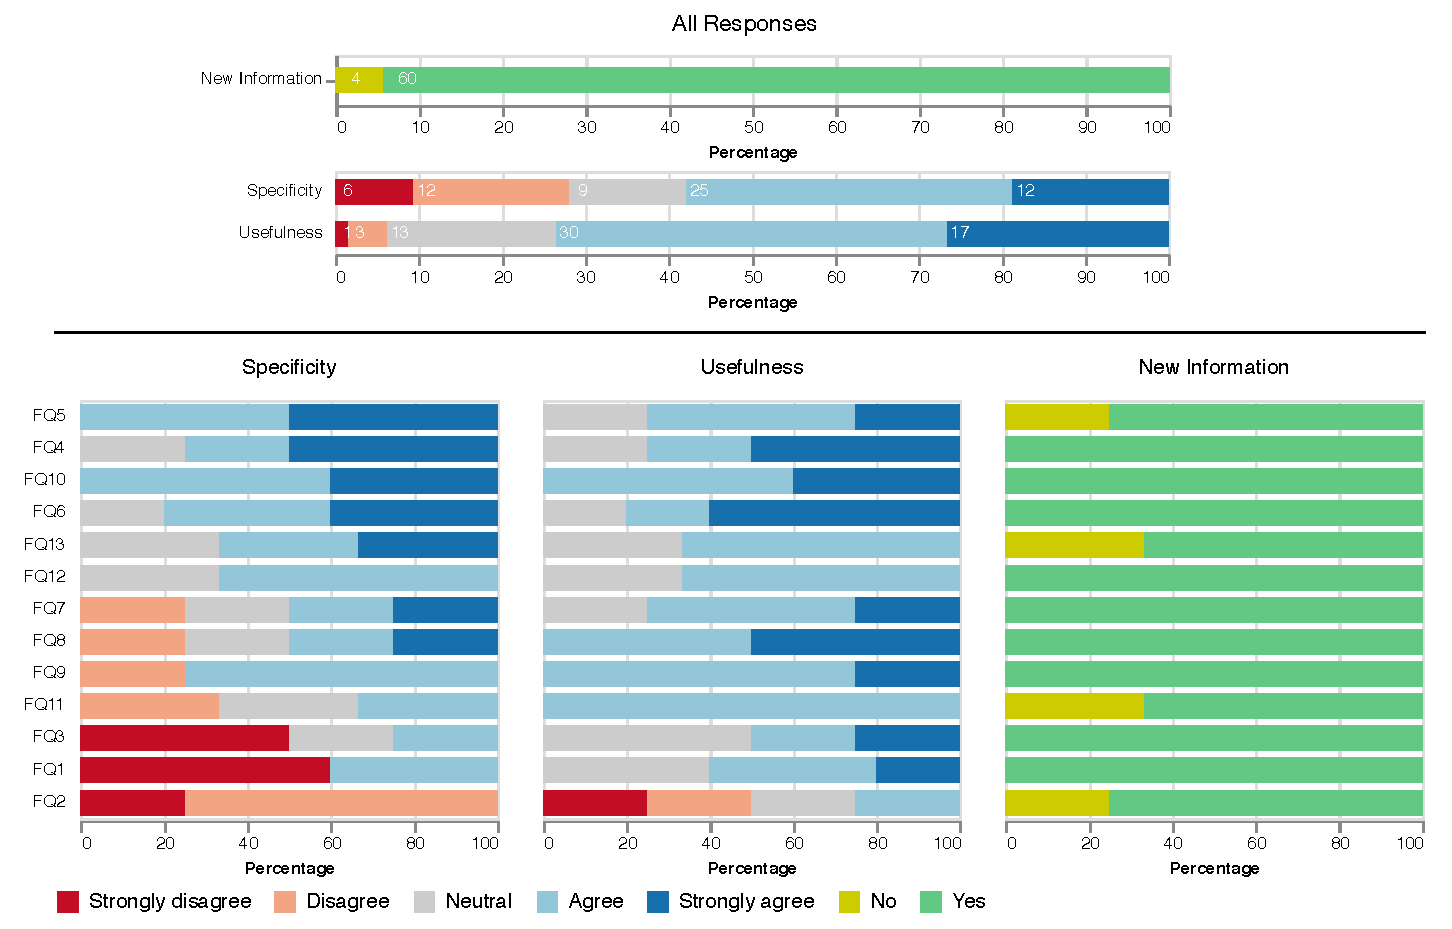
\includegraphics[width=0.99\linewidth]{figures/viz_group.pdf}
\caption{Responses to developer survey grouped per category (top) and per follow-up question (bottom).}
\label{fig:survey}
\end{figure*}

%Results
The survey results showed that out of the 24 different bug report - follow-up question pairs, a majority of participants (at least 3 out of 5) considered 13 follow-up questions as valid, and 11 as invalid. This ratio is analogous to the results we observed for Precision@1 in the held-out set evaluation above, confirming expectations.

The results of the survey, along each dimension, are presented both at the granularity of individual response and at the granularity of a bug report (and follow-up question pair) in Figure~\ref{fig:survey}. The survey results indicate that among categories, the selected follow-up questions by \evpi provide the most of New Information, followed by Usefulness and Specificity. However, all categories were generally positive with over 50\% of all responses on all categories either agreeing or strongly agreeing with the statements on Specificity and Usefulness or affirming that the follow-up question was asking for New Information. Considering the data per follow-up question, in the bottom part of Figure~\ref{fig:survey}, we observe most follow-up questions, which were deemed as valid, were rated positively.  Some follow-up questions have strongly positive ratings, e.g., follow-up question 14 (FQ14) was rated by all 5 respondents as valid, 4/5 agreeing or strongly agreeing that the question was specific, 4/5 agreeing or strongly agreeing that the question was useful, and 5/5 agreeing that the question aimed to provide new information for the bug report.


\subsection{Threats to Validity}


\section{Related Work}
To our knowledge, the proposed approach is the first effort towards improving the quality of bug reports by asking follow-up questions. Prior research related to this area can be broadly grouped into three main categories including evaluation of bug reports quality, approaches for improving deficient bug reports, and techniques automatically posing follow-up questions in domains external to software engineering field.

%bug report quality (focus first on measuring, then on improving)
\noindent
{\em Analyzing the quality of bug reports.} The quality of user written bug reports is a topic that several researchers have been interested in. Linstead et al. applied Latent Dirichlet Analysis to a large corpus of bug reports to study their semantic coherence~\cite{linstead09mining}, while Huo et al. investigated how the  content of a bug report changes depending on the level of expertise of its author~\cite{Huo2014AnES}. Di Sorbo et al. observed that issues marked as ``won't fix'' often contains numerous errors in their reports~\cite{Sorbo2019WontWF}, while insufficient amount of information supplied within a bug report can lead to developers not being able to reproduce as bug, as noted by Joorabchi et al.~\cite{erfani2014works}.
%Kavaler et al. examined language tendencies of bug reports among different developer groups and GitHub projects~\cite{kavaler2017language}.
Researchers have been extensively investigating the content of bug reports to determine the most useful information leading to locating and fixing buggy code efficiently.
%To this end, Bettenburg et al. proposed techniques for automatically identifying stack traces, code snippets, and other structures in bug reports~\cite{bettenburg08extracting}.
To this end, Davies et al. manually analyzed a corpus of bug reports from four popular open-source projects finding that observable behavior and expected behavior are among the most consistently encountered parts of a bug report~\cite{davies14whats}. Survey of software developers conducted by Sasso et al. reveled that steps to reproduce, test cases and stack traces are the most helpful types of information, however they were also the hardest for users to supply~\cite{sasso2016satisficing}. These finding were confirmed and further expanded in the study of Laukkanen et al. who indicated the importance of application's configuration~\cite{laukkanen2011survey}. Chaparro et al. developed a technique leveraging language patterns to automatically extract observable behavior, expected behavior, and steps to reproduce from a bug report~\cite{chaparro17detecting}. Liu et al. proposed to improve Chapparo's technique by eschewing predefined patterns, instead relying on pre-trained classifier to identify steps to reproduce~\cite{liu2020automated}. Recently, Yu et al. developed a tool, S2RMiner, that extracts steps to reproduce from a bug report with high accuracy~\cite{yu2019s2rminer}.
%Karim et al. identified test cases, code examples, steps to reproduce, expected behavior, and stack traces as initially missing features which are often requested~\cite{Karim2017UnderstandingKF, karim2019identifying}.

\noindent
{\em Improving inadequate bug reports.} Researchers have approached the problem of improving the quality of bug reports from a few different angels. One line of work, with numerous proposed techniques, is to detect duplicate bug reports~\cite{sun2011towards,nguyen2012duplicate,chaparro19reformulating}. Another research avenue is to classify bug reports into valid vs. invalid or easy vs. difficult bug reports~\cite{fan20chaff,zhou2016combining,hooimeijer07modeling}. Researchers have also attempted to automatically improve specific parts of bug reports. Moran et al. provided auto-completion for the steps to reproduce portion of bug reports by leveraging image processing of screenshots taken from the application's UI~\cite{moran15autocompleting}.  Chaparro et al. explored how bug report quality can be improved based on unexpected vocabularies in the steps to reproduce~\cite{Chaparro2019AssessingTQ}. Recently proposed BEE tool, implemented as a GitHub plugin, extracts observable behavior, expected behavior, and steps to reproduce from a bug report in order to alert bug reporters when this information is not provided~\cite{song2020bee}.

\noindent
{\em Automatically posing follow-up questions.} Research on automatic question generation has been applied within a few different domains and applications. One topic of extensive prior research is on generating questions from an existing document, i.e., questions whose answers can be found within the given text~\cite{vanderwende2008importance,rus2011question,zhou2017neural,heilman2010good,duan2017question,du2017learning}. For instance, such generated questions can be used for educational assessment and automation. More recently, researchers have envisioned a future where a user's information need will be satisfied via dialog with a virtual assistant, i.e., follow-up questions that are automatically posed to clarify the user's intent. To this end, Braslavski et al. analyzed clarification question patterns on question-answering (QA) websites in order to understand users behavior, and the types of clarification questions asked~\cite{10.1145/3020165.3022149}. Trienes et al. focused on detecting when the original questions in community QA sites are unclear and clarification questions are needed~\cite{trienes2019identifying}. Qu et al. curated and published a large dataset of question and answers intended to help develop conversational search systems~\cite{10.1145/3209978.3210124}. In Web search, follow-up questions have been used for improving document retrieval for low-quality queries~\cite{10.1145/3366423.3380126,10.1145/3331184.3331265,stoyanchev2014towards}. Targeting information that is missing from a document, Rao et al. used generative adversarial neural networks to automatically generate questions that seek to augment Amazon product reviews~\cite{rao-daume-iii-2018-learning}. Asking follow-up questions has been explored in several other contexts such as chatbots~\cite{Hancock2019LearningFD}, open domain question answering systems~\cite{de2005implementing, de2003analysis}, search engines~\cite{Ren2020ConversationsWS}, and image content~\cite{Mostafazadeh_2016}.


\section{Conclusions and Future Work}
In this paper, we have addressed the issue of follow-up questions for inadequate bug reports. We have presented a novel approach of automatically selecting follow-up questions in such cases. To serve our purpose, we have constructed a dataset of 25K bug reports from 6452 unique repositories and generated 10 candidate follow-up questions for each each bug reports. We have used a neural networking approach to sort these questions and evaluated over model with four baselines. The results show that Bug-IQ model is encouraging to come up with a valid follow-up question. 

There are several avenues of future work. First, following Rao et al~\cite{rao2019answer}, we can automatically generate follow-up questions using sequence-to-sequence neutral network model~\cite{sutskever2014sequence, yin2015neural, serban2015building}. Second, Braslavski et al~\cite{10.1145/3020165.3022149}, we can work on generating frequently asked question patterns in bug reports. Third, we can develop a tool and integrate Bug-IQ model in real world platform like GitHub, BugZilla to help the users to point out what type of information may be missing from the original context.


\section*{Acknowledgment}
%The authors acknowledge the help of Sudeep Dharanikota in implementing some of the bug report patterns. This material is based upon work supported by the National Science Foundation under Grant No. (NSF grant number)
Coming soon.

\bibliographystyle{IEEEtran}
\bibliography{paper}

\end{document}
